\documentclass[twoside]{book}

% Packages required by doxygen
\usepackage{fixltx2e}
\usepackage{calc}
\usepackage{doxygen}
\usepackage[export]{adjustbox} % also loads graphicx
\usepackage{graphicx}
\usepackage[utf8]{inputenc}
\usepackage{makeidx}
\usepackage{multicol}
\usepackage{multirow}
\PassOptionsToPackage{warn}{textcomp}
\usepackage{textcomp}
\usepackage[nointegrals]{wasysym}
\usepackage[table]{xcolor}

% Font selection
\usepackage[T1]{fontenc}
\usepackage[scaled=.90]{helvet}
\usepackage{courier}
\usepackage{amssymb}
\usepackage{sectsty}
\renewcommand{\familydefault}{\sfdefault}
\allsectionsfont{%
  \fontseries{bc}\selectfont%
  \color{darkgray}%
}
\renewcommand{\DoxyLabelFont}{%
  \fontseries{bc}\selectfont%
  \color{darkgray}%
}
\newcommand{\+}{\discretionary{\mbox{\scriptsize$\hookleftarrow$}}{}{}}

% Page & text layout
\usepackage{geometry}
\geometry{%
  a4paper,%
  top=2.5cm,%
  bottom=2.5cm,%
  left=2.5cm,%
  right=2.5cm%
}
\tolerance=750
\hfuzz=15pt
\hbadness=750
\setlength{\emergencystretch}{15pt}
\setlength{\parindent}{0cm}
\setlength{\parskip}{0.2cm}
\makeatletter
\renewcommand{\paragraph}{%
  \@startsection{paragraph}{4}{0ex}{-1.0ex}{1.0ex}{%
    \normalfont\normalsize\bfseries\SS@parafont%
  }%
}
\renewcommand{\subparagraph}{%
  \@startsection{subparagraph}{5}{0ex}{-1.0ex}{1.0ex}{%
    \normalfont\normalsize\bfseries\SS@subparafont%
  }%
}
\makeatother

% Headers & footers
\usepackage{fancyhdr}
\pagestyle{fancyplain}
\fancyhead[LE]{\fancyplain{}{\bfseries\thepage}}
\fancyhead[CE]{\fancyplain{}{}}
\fancyhead[RE]{\fancyplain{}{\bfseries\leftmark}}
\fancyhead[LO]{\fancyplain{}{\bfseries\rightmark}}
\fancyhead[CO]{\fancyplain{}{}}
\fancyhead[RO]{\fancyplain{}{\bfseries\thepage}}
\fancyfoot[LE]{\fancyplain{}{}}
\fancyfoot[CE]{\fancyplain{}{}}
\fancyfoot[RE]{\fancyplain{}{\bfseries\scriptsize Generated on Tue Mar 15 2016 11\+:17\+:29 for Space\+Saver by Doxygen }}
\fancyfoot[LO]{\fancyplain{}{\bfseries\scriptsize Generated on Tue Mar 15 2016 11\+:17\+:29 for Space\+Saver by Doxygen }}
\fancyfoot[CO]{\fancyplain{}{}}
\fancyfoot[RO]{\fancyplain{}{}}
\renewcommand{\footrulewidth}{0.4pt}
\renewcommand{\chaptermark}[1]{%
  \markboth{#1}{}%
}
\renewcommand{\sectionmark}[1]{%
  \markright{\thesection\ #1}%
}

% Indices & bibliography
\usepackage{natbib}
\usepackage[titles]{tocloft}
\setcounter{tocdepth}{3}
\setcounter{secnumdepth}{5}
\makeindex

% Hyperlinks (required, but should be loaded last)
\usepackage{ifpdf}
\ifpdf
  \usepackage[pdftex,pagebackref=true]{hyperref}
\else
  \usepackage[ps2pdf,pagebackref=true]{hyperref}
\fi
\hypersetup{%
  colorlinks=true,%
  linkcolor=blue,%
  citecolor=blue,%
  unicode%
}

% Custom commands
\newcommand{\clearemptydoublepage}{%
  \newpage{\pagestyle{empty}\cleardoublepage}%
}


%===== C O N T E N T S =====

\begin{document}

% Titlepage & ToC
\hypersetup{pageanchor=false,
             bookmarks=true,
             bookmarksnumbered=true,
             pdfencoding=unicode
            }
\pagenumbering{roman}
\begin{titlepage}
\vspace*{7cm}
\begin{center}%
{\Large Space\+Saver }\\
\vspace*{1cm}
{\large Generated by Doxygen 1.8.10}\\
\vspace*{0.5cm}
{\small Tue Mar 15 2016 11:17:29}\\
\end{center}
\end{titlepage}
\clearemptydoublepage
\tableofcontents
\clearemptydoublepage
\pagenumbering{arabic}
\hypersetup{pageanchor=true}

%--- Begin generated contents ---
\chapter{Namespace Index}
\section{Packages}
Here are the packages with brief descriptions (if available)\+:\begin{DoxyCompactList}
\item\contentsline{section}{\hyperlink{namespacecourse}{course} }{\pageref{namespacecourse}}{}
\item\contentsline{section}{\hyperlink{namespacecourse_1_1examples}{course.\+examples} }{\pageref{namespacecourse_1_1examples}}{}
\item\contentsline{section}{\hyperlink{namespacecourse_1_1examples_1_1spacesaver}{course.\+examples.\+spacesaver} }{\pageref{namespacecourse_1_1examples_1_1spacesaver}}{}
\end{DoxyCompactList}

\chapter{Hierarchical Index}
\section{Class Hierarchy}
This inheritance list is sorted roughly, but not completely, alphabetically\+:\begin{DoxyCompactList}
\item \contentsline{section}{course.\+examples.\+spacesaver.\+Bmp\+Data}{\pageref{classcourse_1_1examples_1_1spacesaver_1_1_bmp_data}}{}
\item \contentsline{section}{course.\+examples.\+spacesaver.\+Pair}{\pageref{classcourse_1_1examples_1_1spacesaver_1_1_pair}}{}
\item \contentsline{section}{course.\+examples.\+spacesaver.\+Utility}{\pageref{classcourse_1_1examples_1_1spacesaver_1_1_utility}}{}
\item Activity\begin{DoxyCompactList}
\item \contentsline{section}{course.\+examples.\+spacesaver.\+Image\+Viewer}{\pageref{classcourse_1_1examples_1_1spacesaver_1_1_image_viewer}}{}
\item \contentsline{section}{course.\+examples.\+spacesaver.\+Main\+Activity}{\pageref{classcourse_1_1examples_1_1spacesaver_1_1_main_activity}}{}
\end{DoxyCompactList}
\item Base\+Adapter\begin{DoxyCompactList}
\item \contentsline{section}{course.\+examples.\+spacesaver.\+Image\+Adapter}{\pageref{classcourse_1_1examples_1_1spacesaver_1_1_image_adapter}}{}
\end{DoxyCompactList}
\end{DoxyCompactList}

\chapter{Class Index}
\section{Class List}
Here are the classes, structs, unions and interfaces with brief descriptions\+:\begin{DoxyCompactList}
\item\contentsline{section}{\hyperlink{classcourse_1_1examples_1_1spacesaver_1_1_image_adapter}{course.\+examples.\+spacesaver.\+Image\+Adapter} }{\pageref{classcourse_1_1examples_1_1spacesaver_1_1_image_adapter}}{}
\item\contentsline{section}{\hyperlink{classcourse_1_1examples_1_1spacesaver_1_1_main_activity}{course.\+examples.\+spacesaver.\+Main\+Activity} }{\pageref{classcourse_1_1examples_1_1spacesaver_1_1_main_activity}}{}
\item\contentsline{section}{\hyperlink{classcourse_1_1examples_1_1spacesaver_1_1_pair}{course.\+examples.\+spacesaver.\+Pair} }{\pageref{classcourse_1_1examples_1_1spacesaver_1_1_pair}}{}
\item\contentsline{section}{\hyperlink{classcourse_1_1examples_1_1spacesaver_1_1_utility}{course.\+examples.\+spacesaver.\+Utility} }{\pageref{classcourse_1_1examples_1_1spacesaver_1_1_utility}}{}
\end{DoxyCompactList}

\chapter{File Index}
\section{File List}
Here is a list of all files with brief descriptions\+:\begin{DoxyCompactList}
\item\contentsline{section}{app/src/main/java/course/examples/spacesaver/\hyperlink{_image_adapter_8java}{Image\+Adapter.\+java} }{\pageref{_image_adapter_8java}}{}
\item\contentsline{section}{app/src/main/java/course/examples/spacesaver/\hyperlink{_main_activity_8java}{Main\+Activity.\+java} }{\pageref{_main_activity_8java}}{}
\item\contentsline{section}{app/src/main/java/course/examples/spacesaver/\hyperlink{_pair_8java}{Pair.\+java} }{\pageref{_pair_8java}}{}
\item\contentsline{section}{app/src/main/java/course/examples/spacesaver/\hyperlink{_utility_8java}{Utility.\+java} }{\pageref{_utility_8java}}{}
\end{DoxyCompactList}

\chapter{Namespace Documentation}
\hypertarget{namespacecourse}{}\section{Package course}
\label{namespacecourse}\index{course@{course}}
\subsection*{Packages}
\begin{DoxyCompactItemize}
\item 
package \hyperlink{namespacecourse_1_1examples}{examples}
\end{DoxyCompactItemize}

\hypertarget{namespacecourse_1_1examples}{}\section{Package course.\+examples}
\label{namespacecourse_1_1examples}\index{course.\+examples@{course.\+examples}}
\subsection*{Packages}
\begin{DoxyCompactItemize}
\item 
package \hyperlink{namespacecourse_1_1examples_1_1spacesaver}{spacesaver}
\end{DoxyCompactItemize}

\hypertarget{namespacecourse_1_1examples_1_1spacesaver}{}\section{Package course.\+examples.\+spacesaver}
\label{namespacecourse_1_1examples_1_1spacesaver}\index{course.\+examples.\+spacesaver@{course.\+examples.\+spacesaver}}
\subsection*{Classes}
\begin{DoxyCompactItemize}
\item 
class \hyperlink{classcourse_1_1examples_1_1spacesaver_1_1_bmp_data}{Bmp\+Data}
\item 
interface \hyperlink{interfacecourse_1_1examples_1_1spacesaver_1_1_constants}{Constants}
\item 
class \hyperlink{classcourse_1_1examples_1_1spacesaver_1_1_image_adapter}{Image\+Adapter}
\item 
class \hyperlink{classcourse_1_1examples_1_1spacesaver_1_1_image_viewer}{Image\+Viewer}
\item 
class \hyperlink{classcourse_1_1examples_1_1spacesaver_1_1_main_activity}{Main\+Activity}
\item 
class \hyperlink{classcourse_1_1examples_1_1spacesaver_1_1_pair}{Pair}
\item 
class \hyperlink{classcourse_1_1examples_1_1spacesaver_1_1_space_saver_service}{Space\+Saver\+Service}
\item 
class \hyperlink{classcourse_1_1examples_1_1spacesaver_1_1_space_service_receiver}{Space\+Service\+Receiver}
\item 
class \hyperlink{classcourse_1_1examples_1_1spacesaver_1_1_stats_activity}{Stats\+Activity}
\item 
class \hyperlink{classcourse_1_1examples_1_1spacesaver_1_1_utility}{Utility}
\end{DoxyCompactItemize}

\chapter{Class Documentation}
\hypertarget{classcourse_1_1examples_1_1spacesaver_1_1_bmp_data}{}\section{course.\+examples.\+spacesaver.\+Bmp\+Data Class Reference}
\label{classcourse_1_1examples_1_1spacesaver_1_1_bmp_data}\index{course.\+examples.\+spacesaver.\+Bmp\+Data@{course.\+examples.\+spacesaver.\+Bmp\+Data}}


Collaboration diagram for course.\+examples.\+spacesaver.\+Bmp\+Data\+:
\nopagebreak
\begin{figure}[H]
\begin{center}
\leavevmode
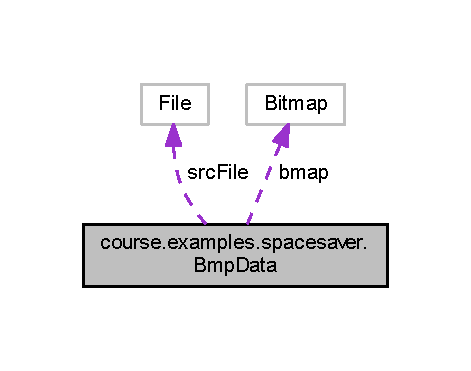
\includegraphics[width=226pt]{classcourse_1_1examples_1_1spacesaver_1_1_bmp_data__coll__graph}
\end{center}
\end{figure}
\subsection*{Public Member Functions}
\begin{DoxyCompactItemize}
\item 
\hyperlink{classcourse_1_1examples_1_1spacesaver_1_1_bmp_data_a833b03c246d444a73e83bea6c9551c5d}{Bmp\+Data} (Bitmap bitmap, File file)
\end{DoxyCompactItemize}


\subsection{Detailed Description}
Wrapper class to hold the path to an image file and its bitmap 

\subsection{Constructor \& Destructor Documentation}
\hypertarget{classcourse_1_1examples_1_1spacesaver_1_1_bmp_data_a833b03c246d444a73e83bea6c9551c5d}{}\index{course\+::examples\+::spacesaver\+::\+Bmp\+Data@{course\+::examples\+::spacesaver\+::\+Bmp\+Data}!Bmp\+Data@{Bmp\+Data}}
\index{Bmp\+Data@{Bmp\+Data}!course\+::examples\+::spacesaver\+::\+Bmp\+Data@{course\+::examples\+::spacesaver\+::\+Bmp\+Data}}
\subsubsection[{Bmp\+Data(\+Bitmap bitmap, File file)}]{\setlength{\rightskip}{0pt plus 5cm}course.\+examples.\+spacesaver.\+Bmp\+Data.\+Bmp\+Data (
\begin{DoxyParamCaption}
\item[{Bitmap}]{bitmap, }
\item[{File}]{file}
\end{DoxyParamCaption}
)}\label{classcourse_1_1examples_1_1spacesaver_1_1_bmp_data_a833b03c246d444a73e83bea6c9551c5d}


The documentation for this class was generated from the following file\+:\begin{DoxyCompactItemize}
\item 
app/src/main/java/course/examples/spacesaver/\hyperlink{_bmp_data_8java}{Bmp\+Data.\+java}\end{DoxyCompactItemize}

\hypertarget{classcourse_1_1examples_1_1spacesaver_1_1_image_adapter}{}\section{course.\+examples.\+spacesaver.\+Image\+Adapter Class Reference}
\label{classcourse_1_1examples_1_1spacesaver_1_1_image_adapter}\index{course.\+examples.\+spacesaver.\+Image\+Adapter@{course.\+examples.\+spacesaver.\+Image\+Adapter}}


Inheritance diagram for course.\+examples.\+spacesaver.\+Image\+Adapter\+:
\nopagebreak
\begin{figure}[H]
\begin{center}
\leavevmode
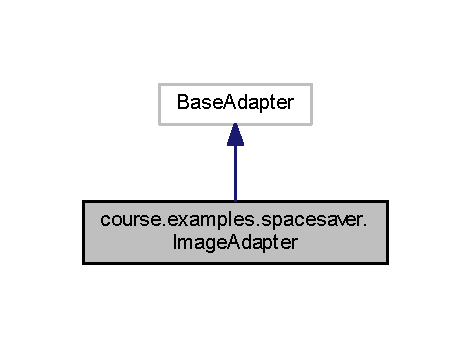
\includegraphics[width=226pt]{classcourse_1_1examples_1_1spacesaver_1_1_image_adapter__inherit__graph}
\end{center}
\end{figure}


Collaboration diagram for course.\+examples.\+spacesaver.\+Image\+Adapter\+:
\nopagebreak
\begin{figure}[H]
\begin{center}
\leavevmode
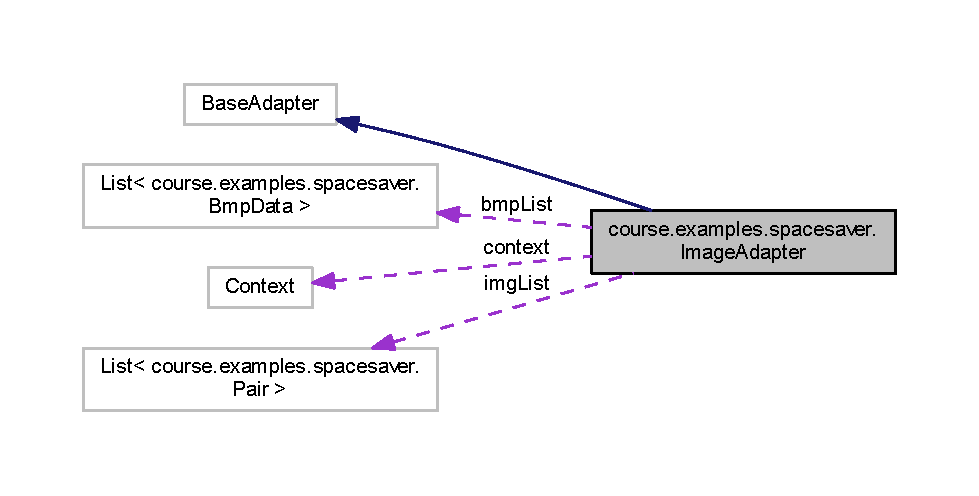
\includegraphics[width=350pt]{classcourse_1_1examples_1_1spacesaver_1_1_image_adapter__coll__graph}
\end{center}
\end{figure}
\subsection*{Public Member Functions}
\begin{DoxyCompactItemize}
\item 
\hyperlink{classcourse_1_1examples_1_1spacesaver_1_1_image_adapter_a4a64ff6f4afb032a7b909d452da4d0f7}{Image\+Adapter} (Context c, List$<$ \hyperlink{classcourse_1_1examples_1_1spacesaver_1_1_pair}{Pair} $>$ list)
\item 
void \hyperlink{classcourse_1_1examples_1_1spacesaver_1_1_image_adapter_a1bc7a805204d8065aaddc2ad1b0c4a1e}{set\+Images} (List$<$ \hyperlink{classcourse_1_1examples_1_1spacesaver_1_1_pair}{Pair} $>$ list)
\item 
int \hyperlink{classcourse_1_1examples_1_1spacesaver_1_1_image_adapter_a7446ece5dd5f5c4f4afeb7a19cdb8728}{get\+Count} ()
\item 
Object \hyperlink{classcourse_1_1examples_1_1spacesaver_1_1_image_adapter_a2011762c7b8bd44e291c1d75ca223581}{get\+Item} (int position)
\item 
long \hyperlink{classcourse_1_1examples_1_1spacesaver_1_1_image_adapter_a54e7407f7a3d8e2e18513e8826ee861e}{get\+Item\+Id} (int position)
\item 
View \hyperlink{classcourse_1_1examples_1_1spacesaver_1_1_image_adapter_a4072f1ec52b57c428c4c85261be15986}{get\+View} (int position, View convert\+View, View\+Group parent)
\end{DoxyCompactItemize}
\subsection*{Static Public Attributes}
\begin{DoxyCompactItemize}
\item 
static final String \hyperlink{classcourse_1_1examples_1_1spacesaver_1_1_image_adapter_a6cf088221e1ed475f35d61db7ff3f4a4}{L\+O\+G\+\_\+\+T\+A\+G\+\_\+\+N\+A\+M\+E} = \char`\"{}Space\+Saver.\+Image\+Adapter\char`\"{}
\end{DoxyCompactItemize}


\subsection{Detailed Description}
Created by kannanb on 3/8/2016. 

\subsection{Constructor \& Destructor Documentation}
\hypertarget{classcourse_1_1examples_1_1spacesaver_1_1_image_adapter_a4a64ff6f4afb032a7b909d452da4d0f7}{}\index{course\+::examples\+::spacesaver\+::\+Image\+Adapter@{course\+::examples\+::spacesaver\+::\+Image\+Adapter}!Image\+Adapter@{Image\+Adapter}}
\index{Image\+Adapter@{Image\+Adapter}!course\+::examples\+::spacesaver\+::\+Image\+Adapter@{course\+::examples\+::spacesaver\+::\+Image\+Adapter}}
\subsubsection[{Image\+Adapter(\+Context c, List$<$ Pair $>$ list)}]{\setlength{\rightskip}{0pt plus 5cm}course.\+examples.\+spacesaver.\+Image\+Adapter.\+Image\+Adapter (
\begin{DoxyParamCaption}
\item[{Context}]{c, }
\item[{List$<$ {\bf Pair} $>$}]{list}
\end{DoxyParamCaption}
)}\label{classcourse_1_1examples_1_1spacesaver_1_1_image_adapter_a4a64ff6f4afb032a7b909d452da4d0f7}


\subsection{Member Function Documentation}
\hypertarget{classcourse_1_1examples_1_1spacesaver_1_1_image_adapter_a7446ece5dd5f5c4f4afeb7a19cdb8728}{}\index{course\+::examples\+::spacesaver\+::\+Image\+Adapter@{course\+::examples\+::spacesaver\+::\+Image\+Adapter}!get\+Count@{get\+Count}}
\index{get\+Count@{get\+Count}!course\+::examples\+::spacesaver\+::\+Image\+Adapter@{course\+::examples\+::spacesaver\+::\+Image\+Adapter}}
\subsubsection[{get\+Count()}]{\setlength{\rightskip}{0pt plus 5cm}int course.\+examples.\+spacesaver.\+Image\+Adapter.\+get\+Count (
\begin{DoxyParamCaption}
{}
\end{DoxyParamCaption}
)}\label{classcourse_1_1examples_1_1spacesaver_1_1_image_adapter_a7446ece5dd5f5c4f4afeb7a19cdb8728}
\hypertarget{classcourse_1_1examples_1_1spacesaver_1_1_image_adapter_a2011762c7b8bd44e291c1d75ca223581}{}\index{course\+::examples\+::spacesaver\+::\+Image\+Adapter@{course\+::examples\+::spacesaver\+::\+Image\+Adapter}!get\+Item@{get\+Item}}
\index{get\+Item@{get\+Item}!course\+::examples\+::spacesaver\+::\+Image\+Adapter@{course\+::examples\+::spacesaver\+::\+Image\+Adapter}}
\subsubsection[{get\+Item(int position)}]{\setlength{\rightskip}{0pt plus 5cm}Object course.\+examples.\+spacesaver.\+Image\+Adapter.\+get\+Item (
\begin{DoxyParamCaption}
\item[{int}]{position}
\end{DoxyParamCaption}
)}\label{classcourse_1_1examples_1_1spacesaver_1_1_image_adapter_a2011762c7b8bd44e291c1d75ca223581}
\hypertarget{classcourse_1_1examples_1_1spacesaver_1_1_image_adapter_a54e7407f7a3d8e2e18513e8826ee861e}{}\index{course\+::examples\+::spacesaver\+::\+Image\+Adapter@{course\+::examples\+::spacesaver\+::\+Image\+Adapter}!get\+Item\+Id@{get\+Item\+Id}}
\index{get\+Item\+Id@{get\+Item\+Id}!course\+::examples\+::spacesaver\+::\+Image\+Adapter@{course\+::examples\+::spacesaver\+::\+Image\+Adapter}}
\subsubsection[{get\+Item\+Id(int position)}]{\setlength{\rightskip}{0pt plus 5cm}long course.\+examples.\+spacesaver.\+Image\+Adapter.\+get\+Item\+Id (
\begin{DoxyParamCaption}
\item[{int}]{position}
\end{DoxyParamCaption}
)}\label{classcourse_1_1examples_1_1spacesaver_1_1_image_adapter_a54e7407f7a3d8e2e18513e8826ee861e}
\hypertarget{classcourse_1_1examples_1_1spacesaver_1_1_image_adapter_a4072f1ec52b57c428c4c85261be15986}{}\index{course\+::examples\+::spacesaver\+::\+Image\+Adapter@{course\+::examples\+::spacesaver\+::\+Image\+Adapter}!get\+View@{get\+View}}
\index{get\+View@{get\+View}!course\+::examples\+::spacesaver\+::\+Image\+Adapter@{course\+::examples\+::spacesaver\+::\+Image\+Adapter}}
\subsubsection[{get\+View(int position, View convert\+View, View\+Group parent)}]{\setlength{\rightskip}{0pt plus 5cm}View course.\+examples.\+spacesaver.\+Image\+Adapter.\+get\+View (
\begin{DoxyParamCaption}
\item[{int}]{position, }
\item[{View}]{convert\+View, }
\item[{View\+Group}]{parent}
\end{DoxyParamCaption}
)}\label{classcourse_1_1examples_1_1spacesaver_1_1_image_adapter_a4072f1ec52b57c428c4c85261be15986}
\hypertarget{classcourse_1_1examples_1_1spacesaver_1_1_image_adapter_a1bc7a805204d8065aaddc2ad1b0c4a1e}{}\index{course\+::examples\+::spacesaver\+::\+Image\+Adapter@{course\+::examples\+::spacesaver\+::\+Image\+Adapter}!set\+Images@{set\+Images}}
\index{set\+Images@{set\+Images}!course\+::examples\+::spacesaver\+::\+Image\+Adapter@{course\+::examples\+::spacesaver\+::\+Image\+Adapter}}
\subsubsection[{set\+Images(\+List$<$ Pair $>$ list)}]{\setlength{\rightskip}{0pt plus 5cm}void course.\+examples.\+spacesaver.\+Image\+Adapter.\+set\+Images (
\begin{DoxyParamCaption}
\item[{List$<$ {\bf Pair} $>$}]{list}
\end{DoxyParamCaption}
)}\label{classcourse_1_1examples_1_1spacesaver_1_1_image_adapter_a1bc7a805204d8065aaddc2ad1b0c4a1e}


\subsection{Member Data Documentation}
\hypertarget{classcourse_1_1examples_1_1spacesaver_1_1_image_adapter_a6cf088221e1ed475f35d61db7ff3f4a4}{}\index{course\+::examples\+::spacesaver\+::\+Image\+Adapter@{course\+::examples\+::spacesaver\+::\+Image\+Adapter}!L\+O\+G\+\_\+\+T\+A\+G\+\_\+\+N\+A\+M\+E@{L\+O\+G\+\_\+\+T\+A\+G\+\_\+\+N\+A\+M\+E}}
\index{L\+O\+G\+\_\+\+T\+A\+G\+\_\+\+N\+A\+M\+E@{L\+O\+G\+\_\+\+T\+A\+G\+\_\+\+N\+A\+M\+E}!course\+::examples\+::spacesaver\+::\+Image\+Adapter@{course\+::examples\+::spacesaver\+::\+Image\+Adapter}}
\subsubsection[{L\+O\+G\+\_\+\+T\+A\+G\+\_\+\+N\+A\+M\+E}]{\setlength{\rightskip}{0pt plus 5cm}final String course.\+examples.\+spacesaver.\+Image\+Adapter.\+L\+O\+G\+\_\+\+T\+A\+G\+\_\+\+N\+A\+M\+E = \char`\"{}Space\+Saver.\+Image\+Adapter\char`\"{}\hspace{0.3cm}{\ttfamily [static]}}\label{classcourse_1_1examples_1_1spacesaver_1_1_image_adapter_a6cf088221e1ed475f35d61db7ff3f4a4}


The documentation for this class was generated from the following file\+:\begin{DoxyCompactItemize}
\item 
app/src/main/java/course/examples/spacesaver/\hyperlink{_image_adapter_8java}{Image\+Adapter.\+java}\end{DoxyCompactItemize}

\hypertarget{classcourse_1_1examples_1_1spacesaver_1_1_image_viewer}{}\section{course.\+examples.\+spacesaver.\+Image\+Viewer Class Reference}
\label{classcourse_1_1examples_1_1spacesaver_1_1_image_viewer}\index{course.\+examples.\+spacesaver.\+Image\+Viewer@{course.\+examples.\+spacesaver.\+Image\+Viewer}}


Inheritance diagram for course.\+examples.\+spacesaver.\+Image\+Viewer\+:
\nopagebreak
\begin{figure}[H]
\begin{center}
\leavevmode
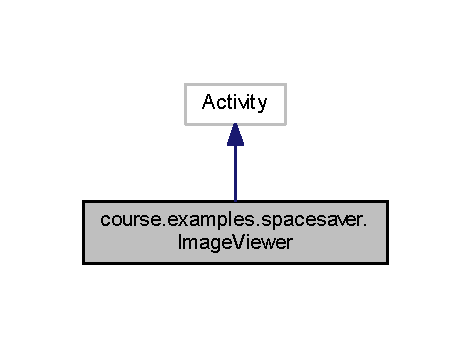
\includegraphics[width=226pt]{classcourse_1_1examples_1_1spacesaver_1_1_image_viewer__inherit__graph}
\end{center}
\end{figure}


Collaboration diagram for course.\+examples.\+spacesaver.\+Image\+Viewer\+:
\nopagebreak
\begin{figure}[H]
\begin{center}
\leavevmode
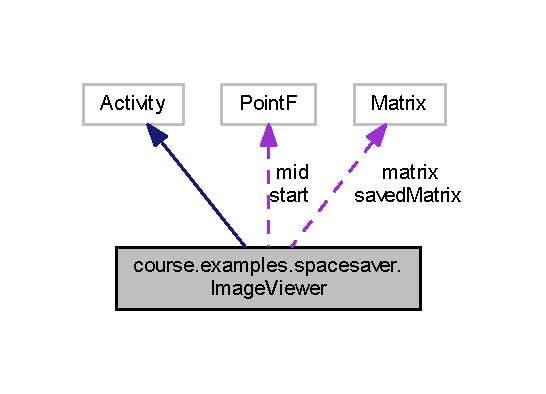
\includegraphics[width=262pt]{classcourse_1_1examples_1_1spacesaver_1_1_image_viewer__coll__graph}
\end{center}
\end{figure}
\subsection*{Public Member Functions}
\begin{DoxyCompactItemize}
\item 
boolean \hyperlink{classcourse_1_1examples_1_1spacesaver_1_1_image_viewer_a1b01127ae6b5efe2d351adbacd678435}{on\+Touch\+Event} (Motion\+Event event)
\end{DoxyCompactItemize}
\subsection*{Static Public Attributes}
\begin{DoxyCompactItemize}
\item 
static final String \hyperlink{classcourse_1_1examples_1_1spacesaver_1_1_image_viewer_af01160015f24efaa8925b71c742633b7}{L\+O\+G\+\_\+\+T\+A\+G\+\_\+\+N\+A\+M\+E} = \char`\"{}Space\+Saver.\+Image\+Viewer\char`\"{}
\end{DoxyCompactItemize}
\subsection*{Protected Member Functions}
\begin{DoxyCompactItemize}
\item 
void \hyperlink{classcourse_1_1examples_1_1spacesaver_1_1_image_viewer_a6bcc20e17948af4e83864323bf8aafd3}{on\+Create} (Bundle saved\+Instance\+State)
\end{DoxyCompactItemize}


\subsection{Detailed Description}
Activity class to render a single image in an Image View alongwith its path on the local storage Created by kannanb on 3/14/2016. 

\subsection{Member Function Documentation}
\hypertarget{classcourse_1_1examples_1_1spacesaver_1_1_image_viewer_a6bcc20e17948af4e83864323bf8aafd3}{}\index{course\+::examples\+::spacesaver\+::\+Image\+Viewer@{course\+::examples\+::spacesaver\+::\+Image\+Viewer}!on\+Create@{on\+Create}}
\index{on\+Create@{on\+Create}!course\+::examples\+::spacesaver\+::\+Image\+Viewer@{course\+::examples\+::spacesaver\+::\+Image\+Viewer}}
\subsubsection[{on\+Create(\+Bundle saved\+Instance\+State)}]{\setlength{\rightskip}{0pt plus 5cm}void course.\+examples.\+spacesaver.\+Image\+Viewer.\+on\+Create (
\begin{DoxyParamCaption}
\item[{Bundle}]{saved\+Instance\+State}
\end{DoxyParamCaption}
)\hspace{0.3cm}{\ttfamily [protected]}}\label{classcourse_1_1examples_1_1spacesaver_1_1_image_viewer_a6bcc20e17948af4e83864323bf8aafd3}
Method to initialize U\+I components of the class and prepare for user interactions . 
\begin{DoxyParams}{Parameters}
{\em saved\+Instance\+State} & \\
\hline
\end{DoxyParams}
\hypertarget{classcourse_1_1examples_1_1spacesaver_1_1_image_viewer_a1b01127ae6b5efe2d351adbacd678435}{}\index{course\+::examples\+::spacesaver\+::\+Image\+Viewer@{course\+::examples\+::spacesaver\+::\+Image\+Viewer}!on\+Touch\+Event@{on\+Touch\+Event}}
\index{on\+Touch\+Event@{on\+Touch\+Event}!course\+::examples\+::spacesaver\+::\+Image\+Viewer@{course\+::examples\+::spacesaver\+::\+Image\+Viewer}}
\subsubsection[{on\+Touch\+Event(\+Motion\+Event event)}]{\setlength{\rightskip}{0pt plus 5cm}boolean course.\+examples.\+spacesaver.\+Image\+Viewer.\+on\+Touch\+Event (
\begin{DoxyParamCaption}
\item[{Motion\+Event}]{event}
\end{DoxyParamCaption}
)}\label{classcourse_1_1examples_1_1spacesaver_1_1_image_viewer_a1b01127ae6b5efe2d351adbacd678435}
Method to handle touch events on the image 
\begin{DoxyParams}{Parameters}
{\em event} & type of touch event triggered (for moving the image, zoom in / zoom out the image) \\
\hline
\end{DoxyParams}
\begin{DoxyReturn}{Returns}
if the event is consumed or not 
\end{DoxyReturn}


\subsection{Member Data Documentation}
\hypertarget{classcourse_1_1examples_1_1spacesaver_1_1_image_viewer_af01160015f24efaa8925b71c742633b7}{}\index{course\+::examples\+::spacesaver\+::\+Image\+Viewer@{course\+::examples\+::spacesaver\+::\+Image\+Viewer}!L\+O\+G\+\_\+\+T\+A\+G\+\_\+\+N\+A\+M\+E@{L\+O\+G\+\_\+\+T\+A\+G\+\_\+\+N\+A\+M\+E}}
\index{L\+O\+G\+\_\+\+T\+A\+G\+\_\+\+N\+A\+M\+E@{L\+O\+G\+\_\+\+T\+A\+G\+\_\+\+N\+A\+M\+E}!course\+::examples\+::spacesaver\+::\+Image\+Viewer@{course\+::examples\+::spacesaver\+::\+Image\+Viewer}}
\subsubsection[{L\+O\+G\+\_\+\+T\+A\+G\+\_\+\+N\+A\+M\+E}]{\setlength{\rightskip}{0pt plus 5cm}final String course.\+examples.\+spacesaver.\+Image\+Viewer.\+L\+O\+G\+\_\+\+T\+A\+G\+\_\+\+N\+A\+M\+E = \char`\"{}Space\+Saver.\+Image\+Viewer\char`\"{}\hspace{0.3cm}{\ttfamily [static]}}\label{classcourse_1_1examples_1_1spacesaver_1_1_image_viewer_af01160015f24efaa8925b71c742633b7}


The documentation for this class was generated from the following file\+:\begin{DoxyCompactItemize}
\item 
app/src/main/java/course/examples/spacesaver/\hyperlink{_image_viewer_8java}{Image\+Viewer.\+java}\end{DoxyCompactItemize}

\hypertarget{classcourse_1_1examples_1_1spacesaver_1_1_main_activity}{}\section{course.\+examples.\+spacesaver.\+Main\+Activity Class Reference}
\label{classcourse_1_1examples_1_1spacesaver_1_1_main_activity}\index{course.\+examples.\+spacesaver.\+Main\+Activity@{course.\+examples.\+spacesaver.\+Main\+Activity}}


Inheritance diagram for course.\+examples.\+spacesaver.\+Main\+Activity\+:
\nopagebreak
\begin{figure}[H]
\begin{center}
\leavevmode
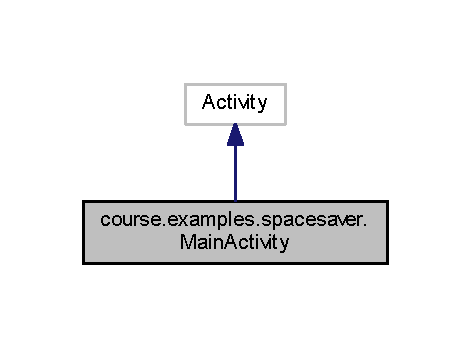
\includegraphics[width=226pt]{classcourse_1_1examples_1_1spacesaver_1_1_main_activity__inherit__graph}
\end{center}
\end{figure}


Collaboration diagram for course.\+examples.\+spacesaver.\+Main\+Activity\+:
\nopagebreak
\begin{figure}[H]
\begin{center}
\leavevmode
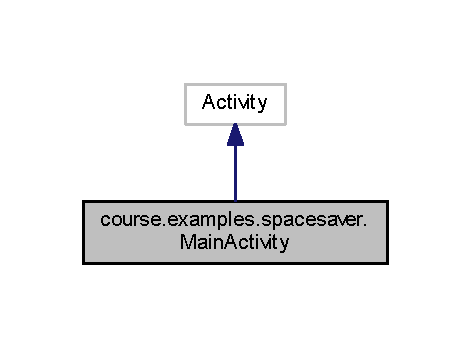
\includegraphics[width=226pt]{classcourse_1_1examples_1_1spacesaver_1_1_main_activity__coll__graph}
\end{center}
\end{figure}
\subsection*{Public Member Functions}
\begin{DoxyCompactItemize}
\item 
boolean \hyperlink{classcourse_1_1examples_1_1spacesaver_1_1_main_activity_a02f312998957aefd4c7a932532e48615}{on\+Create\+Options\+Menu} (Menu menu)
\item 
boolean \hyperlink{classcourse_1_1examples_1_1spacesaver_1_1_main_activity_a819d87dc906ff944c4f60cc044f05498}{on\+Options\+Item\+Selected} (Menu\+Item item)
\end{DoxyCompactItemize}
\subsection*{Static Public Attributes}
\begin{DoxyCompactItemize}
\item 
static final String \hyperlink{classcourse_1_1examples_1_1spacesaver_1_1_main_activity_a62fba147272fa9f0399c82fdd08dbc82}{U\+S\+E\+R\+\_\+\+P\+R\+E\+F\+E\+R\+E\+N\+C\+E} = \char`\"{}User\+Prefs\char`\"{}
\item 
static final String \hyperlink{classcourse_1_1examples_1_1spacesaver_1_1_main_activity_a02332766acdcc44702cbfaee00c0b7ec}{I\+M\+A\+G\+E\+\_\+\+Q\+U\+A\+L\+I\+T\+Y} = \char`\"{}Image\+Quality\char`\"{}
\item 
static final String \hyperlink{classcourse_1_1examples_1_1spacesaver_1_1_main_activity_a73bec883ca93d8c9c0691b1233f08f38}{S\+P\+A\+C\+E\+\_\+\+T\+H\+R\+E\+S\+H\+O\+L\+D} = \char`\"{}Space\+Threshold\char`\"{}
\end{DoxyCompactItemize}
\subsection*{Protected Member Functions}
\begin{DoxyCompactItemize}
\item 
void \hyperlink{classcourse_1_1examples_1_1spacesaver_1_1_main_activity_a03e5171f1ff658442936a03ef4caf7a3}{on\+Create} (Bundle saved\+Instance\+State)
\end{DoxyCompactItemize}


\subsection{Member Function Documentation}
\hypertarget{classcourse_1_1examples_1_1spacesaver_1_1_main_activity_a03e5171f1ff658442936a03ef4caf7a3}{}\index{course\+::examples\+::spacesaver\+::\+Main\+Activity@{course\+::examples\+::spacesaver\+::\+Main\+Activity}!on\+Create@{on\+Create}}
\index{on\+Create@{on\+Create}!course\+::examples\+::spacesaver\+::\+Main\+Activity@{course\+::examples\+::spacesaver\+::\+Main\+Activity}}
\subsubsection[{on\+Create(\+Bundle saved\+Instance\+State)}]{\setlength{\rightskip}{0pt plus 5cm}void course.\+examples.\+spacesaver.\+Main\+Activity.\+on\+Create (
\begin{DoxyParamCaption}
\item[{Bundle}]{saved\+Instance\+State}
\end{DoxyParamCaption}
)\hspace{0.3cm}{\ttfamily [protected]}}\label{classcourse_1_1examples_1_1spacesaver_1_1_main_activity_a03e5171f1ff658442936a03ef4caf7a3}
\hypertarget{classcourse_1_1examples_1_1spacesaver_1_1_main_activity_a02f312998957aefd4c7a932532e48615}{}\index{course\+::examples\+::spacesaver\+::\+Main\+Activity@{course\+::examples\+::spacesaver\+::\+Main\+Activity}!on\+Create\+Options\+Menu@{on\+Create\+Options\+Menu}}
\index{on\+Create\+Options\+Menu@{on\+Create\+Options\+Menu}!course\+::examples\+::spacesaver\+::\+Main\+Activity@{course\+::examples\+::spacesaver\+::\+Main\+Activity}}
\subsubsection[{on\+Create\+Options\+Menu(\+Menu menu)}]{\setlength{\rightskip}{0pt plus 5cm}boolean course.\+examples.\+spacesaver.\+Main\+Activity.\+on\+Create\+Options\+Menu (
\begin{DoxyParamCaption}
\item[{Menu}]{menu}
\end{DoxyParamCaption}
)}\label{classcourse_1_1examples_1_1spacesaver_1_1_main_activity_a02f312998957aefd4c7a932532e48615}
\hypertarget{classcourse_1_1examples_1_1spacesaver_1_1_main_activity_a819d87dc906ff944c4f60cc044f05498}{}\index{course\+::examples\+::spacesaver\+::\+Main\+Activity@{course\+::examples\+::spacesaver\+::\+Main\+Activity}!on\+Options\+Item\+Selected@{on\+Options\+Item\+Selected}}
\index{on\+Options\+Item\+Selected@{on\+Options\+Item\+Selected}!course\+::examples\+::spacesaver\+::\+Main\+Activity@{course\+::examples\+::spacesaver\+::\+Main\+Activity}}
\subsubsection[{on\+Options\+Item\+Selected(\+Menu\+Item item)}]{\setlength{\rightskip}{0pt plus 5cm}boolean course.\+examples.\+spacesaver.\+Main\+Activity.\+on\+Options\+Item\+Selected (
\begin{DoxyParamCaption}
\item[{Menu\+Item}]{item}
\end{DoxyParamCaption}
)}\label{classcourse_1_1examples_1_1spacesaver_1_1_main_activity_a819d87dc906ff944c4f60cc044f05498}


\subsection{Member Data Documentation}
\hypertarget{classcourse_1_1examples_1_1spacesaver_1_1_main_activity_a02332766acdcc44702cbfaee00c0b7ec}{}\index{course\+::examples\+::spacesaver\+::\+Main\+Activity@{course\+::examples\+::spacesaver\+::\+Main\+Activity}!I\+M\+A\+G\+E\+\_\+\+Q\+U\+A\+L\+I\+T\+Y@{I\+M\+A\+G\+E\+\_\+\+Q\+U\+A\+L\+I\+T\+Y}}
\index{I\+M\+A\+G\+E\+\_\+\+Q\+U\+A\+L\+I\+T\+Y@{I\+M\+A\+G\+E\+\_\+\+Q\+U\+A\+L\+I\+T\+Y}!course\+::examples\+::spacesaver\+::\+Main\+Activity@{course\+::examples\+::spacesaver\+::\+Main\+Activity}}
\subsubsection[{I\+M\+A\+G\+E\+\_\+\+Q\+U\+A\+L\+I\+T\+Y}]{\setlength{\rightskip}{0pt plus 5cm}final String course.\+examples.\+spacesaver.\+Main\+Activity.\+I\+M\+A\+G\+E\+\_\+\+Q\+U\+A\+L\+I\+T\+Y = \char`\"{}Image\+Quality\char`\"{}\hspace{0.3cm}{\ttfamily [static]}}\label{classcourse_1_1examples_1_1spacesaver_1_1_main_activity_a02332766acdcc44702cbfaee00c0b7ec}
\hypertarget{classcourse_1_1examples_1_1spacesaver_1_1_main_activity_a73bec883ca93d8c9c0691b1233f08f38}{}\index{course\+::examples\+::spacesaver\+::\+Main\+Activity@{course\+::examples\+::spacesaver\+::\+Main\+Activity}!S\+P\+A\+C\+E\+\_\+\+T\+H\+R\+E\+S\+H\+O\+L\+D@{S\+P\+A\+C\+E\+\_\+\+T\+H\+R\+E\+S\+H\+O\+L\+D}}
\index{S\+P\+A\+C\+E\+\_\+\+T\+H\+R\+E\+S\+H\+O\+L\+D@{S\+P\+A\+C\+E\+\_\+\+T\+H\+R\+E\+S\+H\+O\+L\+D}!course\+::examples\+::spacesaver\+::\+Main\+Activity@{course\+::examples\+::spacesaver\+::\+Main\+Activity}}
\subsubsection[{S\+P\+A\+C\+E\+\_\+\+T\+H\+R\+E\+S\+H\+O\+L\+D}]{\setlength{\rightskip}{0pt plus 5cm}final String course.\+examples.\+spacesaver.\+Main\+Activity.\+S\+P\+A\+C\+E\+\_\+\+T\+H\+R\+E\+S\+H\+O\+L\+D = \char`\"{}Space\+Threshold\char`\"{}\hspace{0.3cm}{\ttfamily [static]}}\label{classcourse_1_1examples_1_1spacesaver_1_1_main_activity_a73bec883ca93d8c9c0691b1233f08f38}
\hypertarget{classcourse_1_1examples_1_1spacesaver_1_1_main_activity_a62fba147272fa9f0399c82fdd08dbc82}{}\index{course\+::examples\+::spacesaver\+::\+Main\+Activity@{course\+::examples\+::spacesaver\+::\+Main\+Activity}!U\+S\+E\+R\+\_\+\+P\+R\+E\+F\+E\+R\+E\+N\+C\+E@{U\+S\+E\+R\+\_\+\+P\+R\+E\+F\+E\+R\+E\+N\+C\+E}}
\index{U\+S\+E\+R\+\_\+\+P\+R\+E\+F\+E\+R\+E\+N\+C\+E@{U\+S\+E\+R\+\_\+\+P\+R\+E\+F\+E\+R\+E\+N\+C\+E}!course\+::examples\+::spacesaver\+::\+Main\+Activity@{course\+::examples\+::spacesaver\+::\+Main\+Activity}}
\subsubsection[{U\+S\+E\+R\+\_\+\+P\+R\+E\+F\+E\+R\+E\+N\+C\+E}]{\setlength{\rightskip}{0pt plus 5cm}final String course.\+examples.\+spacesaver.\+Main\+Activity.\+U\+S\+E\+R\+\_\+\+P\+R\+E\+F\+E\+R\+E\+N\+C\+E = \char`\"{}User\+Prefs\char`\"{}\hspace{0.3cm}{\ttfamily [static]}}\label{classcourse_1_1examples_1_1spacesaver_1_1_main_activity_a62fba147272fa9f0399c82fdd08dbc82}


The documentation for this class was generated from the following file\+:\begin{DoxyCompactItemize}
\item 
app/src/main/java/course/examples/spacesaver/\hyperlink{_main_activity_8java}{Main\+Activity.\+java}\end{DoxyCompactItemize}

\hypertarget{classcourse_1_1examples_1_1spacesaver_1_1_pair}{}\section{course.\+examples.\+spacesaver.\+Pair Class Reference}
\label{classcourse_1_1examples_1_1spacesaver_1_1_pair}\index{course.\+examples.\+spacesaver.\+Pair@{course.\+examples.\+spacesaver.\+Pair}}
\subsection*{Public Member Functions}
\begin{DoxyCompactItemize}
\item 
\hyperlink{classcourse_1_1examples_1_1spacesaver_1_1_pair_a2eb2305cf2296fa29a66ba8dc9b4f87d}{Pair} (String src\+Image, String c\+Image)
\end{DoxyCompactItemize}


\subsection{Detailed Description}
Wrapper class containing absolute path to source image and the compressed image ~\newline
 Created by kannanb on 3/8/2016. 

\subsection{Constructor \& Destructor Documentation}
\hypertarget{classcourse_1_1examples_1_1spacesaver_1_1_pair_a2eb2305cf2296fa29a66ba8dc9b4f87d}{}\index{course\+::examples\+::spacesaver\+::\+Pair@{course\+::examples\+::spacesaver\+::\+Pair}!Pair@{Pair}}
\index{Pair@{Pair}!course\+::examples\+::spacesaver\+::\+Pair@{course\+::examples\+::spacesaver\+::\+Pair}}
\subsubsection[{Pair(\+String src\+Image, String c\+Image)}]{\setlength{\rightskip}{0pt plus 5cm}course.\+examples.\+spacesaver.\+Pair.\+Pair (
\begin{DoxyParamCaption}
\item[{String}]{src\+Image, }
\item[{String}]{c\+Image}
\end{DoxyParamCaption}
)}\label{classcourse_1_1examples_1_1spacesaver_1_1_pair_a2eb2305cf2296fa29a66ba8dc9b4f87d}
Constructor for passing path to source and compressed image 
\begin{DoxyParams}{Parameters}
{\em src\+Image} & Path to the source (original) image \\
\hline
{\em c\+Image} & Path to the compressed image \\
\hline
\end{DoxyParams}


The documentation for this class was generated from the following file\+:\begin{DoxyCompactItemize}
\item 
app/src/main/java/course/examples/spacesaver/\hyperlink{_pair_8java}{Pair.\+java}\end{DoxyCompactItemize}

\hypertarget{classcourse_1_1examples_1_1spacesaver_1_1_utility}{}\section{course.\+examples.\+spacesaver.\+Utility Class Reference}
\label{classcourse_1_1examples_1_1spacesaver_1_1_utility}\index{course.\+examples.\+spacesaver.\+Utility@{course.\+examples.\+spacesaver.\+Utility}}
\subsection*{Static Public Member Functions}
\begin{DoxyCompactItemize}
\item 
static String \hyperlink{classcourse_1_1examples_1_1spacesaver_1_1_utility_afb38a3ff9ea902240c74adad9d975b80}{get\+Bucket\+Id} (String path)
\item 
static List$<$ String $>$ \hyperlink{classcourse_1_1examples_1_1spacesaver_1_1_utility_a7d516823eb324565737ea69a39e604f9}{get\+Camera\+Images} (Context context)
\item 
static void \hyperlink{classcourse_1_1examples_1_1spacesaver_1_1_utility_a534b914baf6a7ef4d7f681a7d56e4da6}{delete\+Images} (List$<$ String $>$ img\+List, int max\+Count)
\item 
static String \hyperlink{classcourse_1_1examples_1_1spacesaver_1_1_utility_a6e99256bde02985ef71df62265c56217}{calculate\+Space\+Saved} (List$<$ \hyperlink{classcourse_1_1examples_1_1spacesaver_1_1_pair}{Pair} $>$ pairs)
\item 
static Array\+List$<$ \hyperlink{classcourse_1_1examples_1_1spacesaver_1_1_pair}{Pair} $>$ \hyperlink{classcourse_1_1examples_1_1spacesaver_1_1_utility_a5029adf50e50346e2bb08bb1557ed064}{compress\+Images} (List$<$ String $>$ img\+List, int image\+Quality)
\item 
static String \hyperlink{classcourse_1_1examples_1_1spacesaver_1_1_utility_a8f1697a3c166596b60f83c21d23162fb}{compress\+Image} (String img\+File, int image\+Quality, String img\+Folder)
\item 
static String \hyperlink{classcourse_1_1examples_1_1spacesaver_1_1_utility_a52b2d0846affd9ee60328055d871f4df}{get\+Storage\+Capacity} ()
\item 
static String \hyperlink{classcourse_1_1examples_1_1spacesaver_1_1_utility_aba39539a00ba3e4d7c74198092926dee}{get\+Size\+In\+String} (long filesize)
\end{DoxyCompactItemize}
\subsection*{Static Public Attributes}
\begin{DoxyCompactItemize}
\item 
static final String \hyperlink{classcourse_1_1examples_1_1spacesaver_1_1_utility_a306cf6f2267973d242405123fc51c775}{L\+O\+G\+\_\+\+T\+A\+G\+\_\+\+N\+A\+M\+E} = \char`\"{}Space\+Saver.\+Utility\char`\"{}
\item 
static final long \hyperlink{classcourse_1_1examples_1_1spacesaver_1_1_utility_a291dacb443d1ba16e25c95b0b436b6ec}{K\+I\+L\+O\+B\+Y\+T\+E} = 1024
\item 
static final int \hyperlink{classcourse_1_1examples_1_1spacesaver_1_1_utility_a8953f2c1e57838e6e76c22071b4e5a02}{M\+A\+X\+\_\+\+I\+M\+A\+G\+E\+S\+\_\+\+T\+O\+\_\+\+C\+O\+M\+P\+R\+E\+S\+S} = 15
\end{DoxyCompactItemize}


\subsection{Detailed Description}
Created by kannanb on 3/7/2016. 

\subsection{Member Function Documentation}
\hypertarget{classcourse_1_1examples_1_1spacesaver_1_1_utility_a6e99256bde02985ef71df62265c56217}{}\index{course\+::examples\+::spacesaver\+::\+Utility@{course\+::examples\+::spacesaver\+::\+Utility}!calculate\+Space\+Saved@{calculate\+Space\+Saved}}
\index{calculate\+Space\+Saved@{calculate\+Space\+Saved}!course\+::examples\+::spacesaver\+::\+Utility@{course\+::examples\+::spacesaver\+::\+Utility}}
\subsubsection[{calculate\+Space\+Saved(\+List$<$ Pair $>$ pairs)}]{\setlength{\rightskip}{0pt plus 5cm}static String course.\+examples.\+spacesaver.\+Utility.\+calculate\+Space\+Saved (
\begin{DoxyParamCaption}
\item[{List$<$ {\bf Pair} $>$}]{pairs}
\end{DoxyParamCaption}
)\hspace{0.3cm}{\ttfamily [static]}}\label{classcourse_1_1examples_1_1spacesaver_1_1_utility_a6e99256bde02985ef71df62265c56217}
\hypertarget{classcourse_1_1examples_1_1spacesaver_1_1_utility_a8f1697a3c166596b60f83c21d23162fb}{}\index{course\+::examples\+::spacesaver\+::\+Utility@{course\+::examples\+::spacesaver\+::\+Utility}!compress\+Image@{compress\+Image}}
\index{compress\+Image@{compress\+Image}!course\+::examples\+::spacesaver\+::\+Utility@{course\+::examples\+::spacesaver\+::\+Utility}}
\subsubsection[{compress\+Image(\+String img\+File, int image\+Quality, String img\+Folder)}]{\setlength{\rightskip}{0pt plus 5cm}static String course.\+examples.\+spacesaver.\+Utility.\+compress\+Image (
\begin{DoxyParamCaption}
\item[{String}]{img\+File, }
\item[{int}]{image\+Quality, }
\item[{String}]{img\+Folder}
\end{DoxyParamCaption}
)\hspace{0.3cm}{\ttfamily [static]}}\label{classcourse_1_1examples_1_1spacesaver_1_1_utility_a8f1697a3c166596b60f83c21d23162fb}
\hypertarget{classcourse_1_1examples_1_1spacesaver_1_1_utility_a5029adf50e50346e2bb08bb1557ed064}{}\index{course\+::examples\+::spacesaver\+::\+Utility@{course\+::examples\+::spacesaver\+::\+Utility}!compress\+Images@{compress\+Images}}
\index{compress\+Images@{compress\+Images}!course\+::examples\+::spacesaver\+::\+Utility@{course\+::examples\+::spacesaver\+::\+Utility}}
\subsubsection[{compress\+Images(\+List$<$ String $>$ img\+List, int image\+Quality)}]{\setlength{\rightskip}{0pt plus 5cm}static Array\+List$<${\bf Pair}$>$ course.\+examples.\+spacesaver.\+Utility.\+compress\+Images (
\begin{DoxyParamCaption}
\item[{List$<$ String $>$}]{img\+List, }
\item[{int}]{image\+Quality}
\end{DoxyParamCaption}
)\hspace{0.3cm}{\ttfamily [static]}}\label{classcourse_1_1examples_1_1spacesaver_1_1_utility_a5029adf50e50346e2bb08bb1557ed064}
\hypertarget{classcourse_1_1examples_1_1spacesaver_1_1_utility_a534b914baf6a7ef4d7f681a7d56e4da6}{}\index{course\+::examples\+::spacesaver\+::\+Utility@{course\+::examples\+::spacesaver\+::\+Utility}!delete\+Images@{delete\+Images}}
\index{delete\+Images@{delete\+Images}!course\+::examples\+::spacesaver\+::\+Utility@{course\+::examples\+::spacesaver\+::\+Utility}}
\subsubsection[{delete\+Images(\+List$<$ String $>$ img\+List, int max\+Count)}]{\setlength{\rightskip}{0pt plus 5cm}static void course.\+examples.\+spacesaver.\+Utility.\+delete\+Images (
\begin{DoxyParamCaption}
\item[{List$<$ String $>$}]{img\+List, }
\item[{int}]{max\+Count}
\end{DoxyParamCaption}
)\hspace{0.3cm}{\ttfamily [static]}}\label{classcourse_1_1examples_1_1spacesaver_1_1_utility_a534b914baf6a7ef4d7f681a7d56e4da6}
\hypertarget{classcourse_1_1examples_1_1spacesaver_1_1_utility_afb38a3ff9ea902240c74adad9d975b80}{}\index{course\+::examples\+::spacesaver\+::\+Utility@{course\+::examples\+::spacesaver\+::\+Utility}!get\+Bucket\+Id@{get\+Bucket\+Id}}
\index{get\+Bucket\+Id@{get\+Bucket\+Id}!course\+::examples\+::spacesaver\+::\+Utility@{course\+::examples\+::spacesaver\+::\+Utility}}
\subsubsection[{get\+Bucket\+Id(\+String path)}]{\setlength{\rightskip}{0pt plus 5cm}static String course.\+examples.\+spacesaver.\+Utility.\+get\+Bucket\+Id (
\begin{DoxyParamCaption}
\item[{String}]{path}
\end{DoxyParamCaption}
)\hspace{0.3cm}{\ttfamily [static]}}\label{classcourse_1_1examples_1_1spacesaver_1_1_utility_afb38a3ff9ea902240c74adad9d975b80}
\hypertarget{classcourse_1_1examples_1_1spacesaver_1_1_utility_a7d516823eb324565737ea69a39e604f9}{}\index{course\+::examples\+::spacesaver\+::\+Utility@{course\+::examples\+::spacesaver\+::\+Utility}!get\+Camera\+Images@{get\+Camera\+Images}}
\index{get\+Camera\+Images@{get\+Camera\+Images}!course\+::examples\+::spacesaver\+::\+Utility@{course\+::examples\+::spacesaver\+::\+Utility}}
\subsubsection[{get\+Camera\+Images(\+Context context)}]{\setlength{\rightskip}{0pt plus 5cm}static List$<$String$>$ course.\+examples.\+spacesaver.\+Utility.\+get\+Camera\+Images (
\begin{DoxyParamCaption}
\item[{Context}]{context}
\end{DoxyParamCaption}
)\hspace{0.3cm}{\ttfamily [static]}}\label{classcourse_1_1examples_1_1spacesaver_1_1_utility_a7d516823eb324565737ea69a39e604f9}
\hypertarget{classcourse_1_1examples_1_1spacesaver_1_1_utility_aba39539a00ba3e4d7c74198092926dee}{}\index{course\+::examples\+::spacesaver\+::\+Utility@{course\+::examples\+::spacesaver\+::\+Utility}!get\+Size\+In\+String@{get\+Size\+In\+String}}
\index{get\+Size\+In\+String@{get\+Size\+In\+String}!course\+::examples\+::spacesaver\+::\+Utility@{course\+::examples\+::spacesaver\+::\+Utility}}
\subsubsection[{get\+Size\+In\+String(long filesize)}]{\setlength{\rightskip}{0pt plus 5cm}static String course.\+examples.\+spacesaver.\+Utility.\+get\+Size\+In\+String (
\begin{DoxyParamCaption}
\item[{long}]{filesize}
\end{DoxyParamCaption}
)\hspace{0.3cm}{\ttfamily [static]}}\label{classcourse_1_1examples_1_1spacesaver_1_1_utility_aba39539a00ba3e4d7c74198092926dee}
\hypertarget{classcourse_1_1examples_1_1spacesaver_1_1_utility_a52b2d0846affd9ee60328055d871f4df}{}\index{course\+::examples\+::spacesaver\+::\+Utility@{course\+::examples\+::spacesaver\+::\+Utility}!get\+Storage\+Capacity@{get\+Storage\+Capacity}}
\index{get\+Storage\+Capacity@{get\+Storage\+Capacity}!course\+::examples\+::spacesaver\+::\+Utility@{course\+::examples\+::spacesaver\+::\+Utility}}
\subsubsection[{get\+Storage\+Capacity()}]{\setlength{\rightskip}{0pt plus 5cm}static String course.\+examples.\+spacesaver.\+Utility.\+get\+Storage\+Capacity (
\begin{DoxyParamCaption}
{}
\end{DoxyParamCaption}
)\hspace{0.3cm}{\ttfamily [static]}}\label{classcourse_1_1examples_1_1spacesaver_1_1_utility_a52b2d0846affd9ee60328055d871f4df}


\subsection{Member Data Documentation}
\hypertarget{classcourse_1_1examples_1_1spacesaver_1_1_utility_a291dacb443d1ba16e25c95b0b436b6ec}{}\index{course\+::examples\+::spacesaver\+::\+Utility@{course\+::examples\+::spacesaver\+::\+Utility}!K\+I\+L\+O\+B\+Y\+T\+E@{K\+I\+L\+O\+B\+Y\+T\+E}}
\index{K\+I\+L\+O\+B\+Y\+T\+E@{K\+I\+L\+O\+B\+Y\+T\+E}!course\+::examples\+::spacesaver\+::\+Utility@{course\+::examples\+::spacesaver\+::\+Utility}}
\subsubsection[{K\+I\+L\+O\+B\+Y\+T\+E}]{\setlength{\rightskip}{0pt plus 5cm}final long course.\+examples.\+spacesaver.\+Utility.\+K\+I\+L\+O\+B\+Y\+T\+E = 1024\hspace{0.3cm}{\ttfamily [static]}}\label{classcourse_1_1examples_1_1spacesaver_1_1_utility_a291dacb443d1ba16e25c95b0b436b6ec}
\hypertarget{classcourse_1_1examples_1_1spacesaver_1_1_utility_a306cf6f2267973d242405123fc51c775}{}\index{course\+::examples\+::spacesaver\+::\+Utility@{course\+::examples\+::spacesaver\+::\+Utility}!L\+O\+G\+\_\+\+T\+A\+G\+\_\+\+N\+A\+M\+E@{L\+O\+G\+\_\+\+T\+A\+G\+\_\+\+N\+A\+M\+E}}
\index{L\+O\+G\+\_\+\+T\+A\+G\+\_\+\+N\+A\+M\+E@{L\+O\+G\+\_\+\+T\+A\+G\+\_\+\+N\+A\+M\+E}!course\+::examples\+::spacesaver\+::\+Utility@{course\+::examples\+::spacesaver\+::\+Utility}}
\subsubsection[{L\+O\+G\+\_\+\+T\+A\+G\+\_\+\+N\+A\+M\+E}]{\setlength{\rightskip}{0pt plus 5cm}final String course.\+examples.\+spacesaver.\+Utility.\+L\+O\+G\+\_\+\+T\+A\+G\+\_\+\+N\+A\+M\+E = \char`\"{}Space\+Saver.\+Utility\char`\"{}\hspace{0.3cm}{\ttfamily [static]}}\label{classcourse_1_1examples_1_1spacesaver_1_1_utility_a306cf6f2267973d242405123fc51c775}
\hypertarget{classcourse_1_1examples_1_1spacesaver_1_1_utility_a8953f2c1e57838e6e76c22071b4e5a02}{}\index{course\+::examples\+::spacesaver\+::\+Utility@{course\+::examples\+::spacesaver\+::\+Utility}!M\+A\+X\+\_\+\+I\+M\+A\+G\+E\+S\+\_\+\+T\+O\+\_\+\+C\+O\+M\+P\+R\+E\+S\+S@{M\+A\+X\+\_\+\+I\+M\+A\+G\+E\+S\+\_\+\+T\+O\+\_\+\+C\+O\+M\+P\+R\+E\+S\+S}}
\index{M\+A\+X\+\_\+\+I\+M\+A\+G\+E\+S\+\_\+\+T\+O\+\_\+\+C\+O\+M\+P\+R\+E\+S\+S@{M\+A\+X\+\_\+\+I\+M\+A\+G\+E\+S\+\_\+\+T\+O\+\_\+\+C\+O\+M\+P\+R\+E\+S\+S}!course\+::examples\+::spacesaver\+::\+Utility@{course\+::examples\+::spacesaver\+::\+Utility}}
\subsubsection[{M\+A\+X\+\_\+\+I\+M\+A\+G\+E\+S\+\_\+\+T\+O\+\_\+\+C\+O\+M\+P\+R\+E\+S\+S}]{\setlength{\rightskip}{0pt plus 5cm}final int course.\+examples.\+spacesaver.\+Utility.\+M\+A\+X\+\_\+\+I\+M\+A\+G\+E\+S\+\_\+\+T\+O\+\_\+\+C\+O\+M\+P\+R\+E\+S\+S = 15\hspace{0.3cm}{\ttfamily [static]}}\label{classcourse_1_1examples_1_1spacesaver_1_1_utility_a8953f2c1e57838e6e76c22071b4e5a02}


The documentation for this class was generated from the following file\+:\begin{DoxyCompactItemize}
\item 
app/src/main/java/course/examples/spacesaver/\hyperlink{_utility_8java}{Utility.\+java}\end{DoxyCompactItemize}

\chapter{File Documentation}
\hypertarget{_bmp_data_8java}{}\section{app/src/main/java/course/examples/spacesaver/\+Bmp\+Data.java File Reference}
\label{_bmp_data_8java}\index{app/src/main/java/course/examples/spacesaver/\+Bmp\+Data.\+java@{app/src/main/java/course/examples/spacesaver/\+Bmp\+Data.\+java}}
\subsection*{Classes}
\begin{DoxyCompactItemize}
\item 
class \hyperlink{classcourse_1_1examples_1_1spacesaver_1_1_bmp_data}{course.\+examples.\+spacesaver.\+Bmp\+Data}
\end{DoxyCompactItemize}
\subsection*{Packages}
\begin{DoxyCompactItemize}
\item 
package \hyperlink{namespacecourse_1_1examples_1_1spacesaver}{course.\+examples.\+spacesaver}
\end{DoxyCompactItemize}

\hypertarget{_image_adapter_8java}{}\section{app/src/main/java/course/examples/spacesaver/\+Image\+Adapter.java File Reference}
\label{_image_adapter_8java}\index{app/src/main/java/course/examples/spacesaver/\+Image\+Adapter.\+java@{app/src/main/java/course/examples/spacesaver/\+Image\+Adapter.\+java}}
\subsection*{Classes}
\begin{DoxyCompactItemize}
\item 
class \hyperlink{classcourse_1_1examples_1_1spacesaver_1_1_image_adapter}{course.\+examples.\+spacesaver.\+Image\+Adapter}
\end{DoxyCompactItemize}
\subsection*{Packages}
\begin{DoxyCompactItemize}
\item 
package \hyperlink{namespacecourse_1_1examples_1_1spacesaver}{course.\+examples.\+spacesaver}
\end{DoxyCompactItemize}

\hypertarget{_image_viewer_8java}{}\section{app/src/main/java/course/examples/spacesaver/\+Image\+Viewer.java File Reference}
\label{_image_viewer_8java}\index{app/src/main/java/course/examples/spacesaver/\+Image\+Viewer.\+java@{app/src/main/java/course/examples/spacesaver/\+Image\+Viewer.\+java}}
\subsection*{Classes}
\begin{DoxyCompactItemize}
\item 
class \hyperlink{classcourse_1_1examples_1_1spacesaver_1_1_image_viewer}{course.\+examples.\+spacesaver.\+Image\+Viewer}
\end{DoxyCompactItemize}
\subsection*{Packages}
\begin{DoxyCompactItemize}
\item 
package \hyperlink{namespacecourse_1_1examples_1_1spacesaver}{course.\+examples.\+spacesaver}
\end{DoxyCompactItemize}

\hypertarget{_main_activity_8java}{}\section{app/src/main/java/course/examples/spacesaver/\+Main\+Activity.java File Reference}
\label{_main_activity_8java}\index{app/src/main/java/course/examples/spacesaver/\+Main\+Activity.\+java@{app/src/main/java/course/examples/spacesaver/\+Main\+Activity.\+java}}
\subsection*{Classes}
\begin{DoxyCompactItemize}
\item 
class \hyperlink{classcourse_1_1examples_1_1spacesaver_1_1_main_activity}{course.\+examples.\+spacesaver.\+Main\+Activity}
\end{DoxyCompactItemize}
\subsection*{Packages}
\begin{DoxyCompactItemize}
\item 
package \hyperlink{namespacecourse_1_1examples_1_1spacesaver}{course.\+examples.\+spacesaver}
\end{DoxyCompactItemize}

\hypertarget{_pair_8java}{}\section{app/src/main/java/course/examples/spacesaver/\+Pair.java File Reference}
\label{_pair_8java}\index{app/src/main/java/course/examples/spacesaver/\+Pair.\+java@{app/src/main/java/course/examples/spacesaver/\+Pair.\+java}}
\subsection*{Classes}
\begin{DoxyCompactItemize}
\item 
class \hyperlink{classcourse_1_1examples_1_1spacesaver_1_1_pair}{course.\+examples.\+spacesaver.\+Pair}
\end{DoxyCompactItemize}
\subsection*{Packages}
\begin{DoxyCompactItemize}
\item 
package \hyperlink{namespacecourse_1_1examples_1_1spacesaver}{course.\+examples.\+spacesaver}
\end{DoxyCompactItemize}

\hypertarget{_utility_8java}{}\section{app/src/main/java/course/examples/spacesaver/\+Utility.java File Reference}
\label{_utility_8java}\index{app/src/main/java/course/examples/spacesaver/\+Utility.\+java@{app/src/main/java/course/examples/spacesaver/\+Utility.\+java}}
\subsection*{Classes}
\begin{DoxyCompactItemize}
\item 
class \hyperlink{classcourse_1_1examples_1_1spacesaver_1_1_utility}{course.\+examples.\+spacesaver.\+Utility}
\end{DoxyCompactItemize}
\subsection*{Packages}
\begin{DoxyCompactItemize}
\item 
package \hyperlink{namespacecourse_1_1examples_1_1spacesaver}{course.\+examples.\+spacesaver}
\end{DoxyCompactItemize}

%--- End generated contents ---

% Index
\backmatter
\newpage
\phantomsection
\clearemptydoublepage
\addcontentsline{toc}{chapter}{Index}
\printindex

\end{document}
